\documentclass[11pt,a4paper]{article}
\usepackage[margin=2cm]{geometry}
\usepackage[T1]{fontenc}
\usepackage[utf8]{inputenc}
\usepackage{hyperref}
\usepackage{graphicx}
\usepackage{xcolor}
\usepackage{listings}
\usepackage{tikz}
\usetikzlibrary{positioning,arrows.meta,fit,calc}
\definecolor{codebg}{RGB}{248,250,252}
\definecolor{codeblue}{RGB}{37,99,235}
\definecolor{codegreen}{RGB}{22,101,52}
\definecolor{codered}{RGB}{185,28,28}
\definecolor{codegray}{RGB}{100,116,139}
\definecolor{codeink}{RGB}{30,64,175}
\definecolor{codepurple}{RGB}{126,34,206}
\definecolor{codeorange}{RGB}{194,65,12}
\definecolor{codeslate}{RGB}{51,65,85}
\lstdefinelanguage{JavaScript}{morekeywords={const,let,var,async,await,function,try,catch,return,if,else,for,of,require,module,exports},sensitive=true,morecomment=[l]{//},morestring=[b]",morestring=[b]`}
\lstdefinestyle{prokuraCode}{basicstyle=\ttfamily\small\color{codeink},breaklines=true,frame=single,columns=fullflexible,keepspaces=true,showspaces=false,showstringspaces=false,showtabs=false,tabsize=2,numbers=left,numberstyle=\tiny\color{codegray},keywordstyle=\color{codepurple}\bfseries,stringstyle=\color{codeorange},commentstyle=\color{codegreen}\itshape,identifierstyle=\color{codeink},rulecolor=\color{codeblue},backgroundcolor=\color{codebg},emphstyle=\color{codered}\bfseries,captionpos=b}
\lstset{style=prokuraCode}
\newcommand{\demoscreenshot}[2]{
\begin{figure}[htbp]
\centering
\includegraphics[width=0.92\linewidth,height=0.58\textheight,keepaspectratio]{#1}
\caption{#2}
\end{figure}
}
\newcommand{\validationdiagram}{
\begin{center}
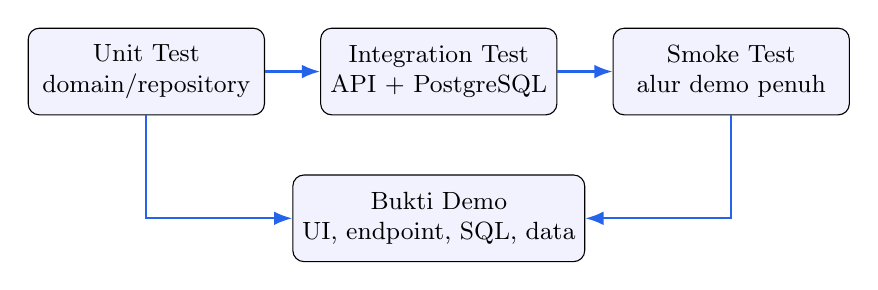
\begin{tikzpicture}[stage/.style={draw, rounded corners, fill=blue!5, align=center, font=\small, minimum width=3.0cm, minimum height=1.1cm}, rel/.style={-Latex, thick, draw=codeblue}]
\node[stage] (unit) {Unit Test\\domain/repository};
\node[stage, right=0.7cm of unit] (integration) {Integration Test\\API + PostgreSQL};
\node[stage, right=0.7cm of integration] (smoke) {Smoke Test\\alur demo penuh};
\node[stage, below=0.75cm of integration] (evidence) {Bukti Demo\\UI, endpoint, SQL, data};
\draw[rel] (unit) -- (integration);
\draw[rel] (integration) -- (smoke);
\draw[rel] (smoke) |- (evidence);
\draw[rel] (unit) |- (evidence);
\end{tikzpicture}
\end{center}
}
\newcommand{\featureflow}[4]{
\begin{center}
\begin{tikzpicture}[flowbox/.style={draw=codeblue, rounded corners=3pt, fill=codebg, align=center, font=\small, text width=2.85cm, minimum height=1.15cm, inner sep=5pt}, flowarrow/.style={-Latex, thick, draw=codeblue}]
\node[flowbox] (ui) {#1};
\node[flowbox, right=0.6cm of ui] (api) {#2};
\node[flowbox, right=0.6cm of api] (db) {#3};
\node[flowbox, right=0.6cm of db] (result) {#4};
\draw[flowarrow] (ui) -- (api);
\draw[flowarrow] (api) -- (db);
\draw[flowarrow] (db) -- (result);
\end{tikzpicture}
\end{center}
}

\newcommand{\docheader}[2]{
\begin{titlepage}
\centering
{\Large\bfseries Prokura HoReCa Supply\par}
\vspace{0.4cm}
{\large Dokumentasi Fitur Microservice Final Project\par}
\vspace{0.8cm}
{\large Workshop Implementasi Rekayasa Perangkat Lunak\par}
\vspace{1.2cm}
{\large\bfseries #1\par}
{\large NIM: #2\par}
\vspace{0.7cm}

\includegraphics[width=4.0cm]{../screenshots/ugm-logo.png}\par
\vspace{0.5cm}
\vfill
{\large Ilmu Komputer\par}
{\large Departemen Ilmu Komputer dan Elektronika (DIKE)\par}
{\large Fakultas Matematika dan Ilmu Pengetahuan Alam\par}
{\large Universitas Gadjah Mada\par}
\vfill
\end{titlepage}
}

\begin{document}
\docheader{Aloysius Pijar Hutama Indrianto}{24/534591/PA/22675}

\section*{Peran}
Owner Inventory Service. Aloysius bertanggung jawab pada perubahan stok gudang dan audit trail pergerakan stok.

\section*{Bukti Microservice}
Inventory Service sudah dipisahkan pada \path{prokura-api/src/services/inventory}. Service ini dapat berjalan sendiri melalui registry di \path{prokura-api/src/service-host.js}.

\begin{lstlisting}[language=JavaScript]
const serviceRegistry = {
  catalog: registerCatalogRoutes,
  customer: registerCustomerRoutes,
  inventory: registerInventoryRoutes,
  order: registerOrderRoutes,
  reporting: registerReportingRoutes,
};
\end{lstlisting}

Penjelasan: entry \texttt{inventory: registerInventoryRoutes} menunjukkan route inventory dipasang sebagai service tersendiri. Pada Docker Compose microservices, service ini diekspos pada port \texttt{5102} dengan health endpoint \texttt{/health}.

\section*{Tanggung Jawab Fitur}
\begin{enumerate}
\item Penambahan stok barang.
\item Riwayat pergerakan stok.
\end{enumerate}

\section*{Diagram Scenario Flow Fitur}
\subsection*{Penambahan stok barang}
\featureflow{Admin memilih produk\\dan jumlah restock}{Inventory Service\\\texttt{PATCH /api/products/:id/stock}}{Update stok\\dan insert movement}{Stok bertambah\\di dashboard}

\subsection*{Riwayat pergerakan stok}
\featureflow{Admin membuka\\riwayat stok}{Inventory Service\\\texttt{GET /api/inventory/movements}}{Query \texttt{inventory\_movements}\\join produk}{Tabel audit stok\\ditampilkan}


\section*{Diagram Tabel yang Ditangani}
\begin{center}
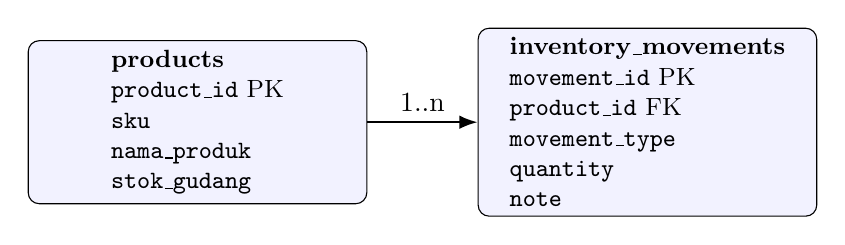
\begin{tikzpicture}[entity/.style={draw, rounded corners, fill=blue!5, align=left, font=\small, minimum width=4.3cm}, rel/.style={-Latex, thick}]
\node[entity] (products) {\textbf{products}\\\texttt{product\_id} PK\\\texttt{sku}\\\texttt{nama\_produk}\\\texttt{stok\_gudang}};
\node[entity, right=1.4cm of products] (movements) {\textbf{inventory\_movements}\\\texttt{movement\_id} PK\\\texttt{product\_id} FK\\\texttt{movement\_type}\\\texttt{quantity}\\\texttt{note}};
\draw[rel] (products) -- node[above]{1..n} (movements);
\end{tikzpicture}
\end{center}

Penjelasan: Inventory Service mengubah \texttt{products.stok\_gudang} dan mencatat setiap perubahan ke \texttt{inventory\_movements}. Relasi \texttt{product\_id} menjaga setiap movement selalu terhubung ke produk yang valid.

\section*{Lokasi Kode Program dan Penjelasan}
\subsection*{Route penambahan stok}
Lokasi kode: \path{prokura-api/src/services/inventory/routes.js}. \texttt{PATCH /api/products/:product\_id/stock}: line 4.

\begin{lstlisting}[language=JavaScript]
app.patch("/api/products/:product_id/stock", async (req, res) => {
  const client = await pool.connect();
  try {
    const { product_id } = req.params;
    const { quantity, note } = req.body;
    let amount;

    try {
      amount = parsePositiveInteger(quantity, "Quantity stok masuk");
    } catch (error) {
      return res.status(400).json({ success: false, message: error.message });
    }
\end{lstlisting}

Penjelasan: endpoint menerima \texttt{product\_id}, \texttt{quantity}, dan catatan. \texttt{parsePositiveInteger} memastikan jumlah stok masuk valid dan positif sebelum database diubah.

\begin{lstlisting}[language=JavaScript]
await client.query("BEGIN");
const { rows } = await client.query(
  `
    UPDATE products
    SET stok_gudang = stok_gudang + $1
    WHERE product_id = $2
    RETURNING product_id, sku, nama_produk, kategori, satuan, harga_dasar, stok_gudang
  `,
  [amount, product_id],
);
\end{lstlisting}

Penjelasan: stok produk bertambah secara atomik dengan parameter \texttt{\$1} untuk jumlah dan \texttt{\$2} untuk produk. \texttt{RETURNING} mengembalikan stok terbaru ke UI.

\begin{lstlisting}[language=JavaScript]
await recordInventoryMovement(client, {
  productId: Number(product_id),
  movementType: "STOCK_IN",
  quantity: amount,
  note: note || "Penambahan stok manual",
  referenceType: "PRODUCT",
  referenceId: Number(product_id),
});

await client.query("COMMIT");
res.json({ success: true, data: rows[0] });
\end{lstlisting}

Penjelasan: setelah stok naik, sistem membuat movement \texttt{STOCK\_IN}. Update stok dan insert movement berada dalam transaksi yang sama agar data stok dan audit trail konsisten.

\subsection*{Route riwayat pergerakan stok}
Lokasi kode: \path{prokura-api/src/services/inventory/routes.js}. \texttt{GET /api/inventory/movements}: line 51.

\begin{lstlisting}[language=JavaScript]
if (req.query.product_id) {
  params.push(req.query.product_id);
  conditions.push(`m.product_id = $${params.length}`);
}

if (req.query.movement_type) {
  params.push(req.query.movement_type);
  conditions.push(`m.movement_type = $${params.length}`);
}
\end{lstlisting}

Penjelasan: endpoint riwayat dapat difilter berdasarkan produk dan tipe movement. Filter ini berguna saat demo untuk menunjukkan riwayat hanya dari produk yang sedang diuji.

\begin{lstlisting}[language=JavaScript]
const { rows } = await pool.query(
  `
    SELECT m.movement_id, m.product_id, p.sku, p.nama_produk,
           m.movement_type, m.quantity, m.note,
           m.reference_type, m.reference_id, m.created_at
    FROM inventory_movements m
    JOIN products p ON m.product_id = p.product_id
    ${where}
    ORDER BY m.created_at DESC, m.movement_id DESC
  `,
  params,
);
\end{lstlisting}

Penjelasan: query mengambil movement dan data produk terkait. Urutan descending membuat movement terbaru muncul paling atas.

\subsection*{SQL insert movement}
Lokasi kode: \path{prokura-api/src/services/inventory/repository.js}. Insert movement: line 22.

\begin{lstlisting}[language=JavaScript]
await client.query(
  `
    INSERT INTO inventory_movements
      (product_id, movement_type, quantity, note, reference_type, reference_id)
    VALUES ($1, $2, $3, $4, $5, $6)
  `,
  [
    movement.productId,
    movement.movementType,
    movement.quantity,
    movement.note,
    movement.referenceType,
    movement.referenceId,
  ],
);
\end{lstlisting}

Penjelasan: repository ini menjadi satu tempat pencatatan movement untuk stok awal, stok masuk, stok keluar, dan stok return. Karena dipakai oleh Catalog dan Order juga, audit inventory tetap konsisten lintas service.

\subsection*{UI admin stok}
Lokasi kode: \path{prokura-admin/app3.py}; menu \texttt{Manajemen Stok Gudang}: line 399, form \texttt{Penambahan Stok Barang}: line 587, tabel \texttt{Riwayat Pergerakan Stok}: line 624.

Penjelasan: UI admin memanggil API inventory untuk menambah stok dan membaca riwayat. Admin tidak menjalankan SQL langsung dari Streamlit.

\section*{SQL Query Demo dan Penjelasan}
\subsection*{Query 1: tambah stok}
\begin{lstlisting}[language=SQL]
UPDATE products
SET stok_gudang = stok_gudang + 25
WHERE product_id = 1
RETURNING product_id, sku, nama_produk, stok_gudang;
\end{lstlisting}
Penjelasan: query ini menambah stok produk dengan \texttt{product\_id = 1} sebanyak 25. \texttt{RETURNING} menunjukkan stok akhir setelah update.

\subsection*{Query 2: catat movement}
\begin{lstlisting}[language=SQL]
INSERT INTO inventory_movements
  (product_id, movement_type, quantity, note, reference_type, reference_id)
VALUES
  (1, 'STOCK_IN', 25, 'Restock demo presentasi', 'PRODUCT', 1);
\end{lstlisting}
Penjelasan: query ini mencatat perubahan stok sebagai movement \texttt{STOCK\_IN}. Data ini menjadi bukti audit bahwa stok bertambah karena restock manual.

\subsection*{Query 3: lihat riwayat movement}
\begin{lstlisting}[language=SQL]
SELECT m.movement_id, m.product_id, p.sku, p.nama_produk,
       m.movement_type, m.quantity, m.note,
       m.reference_type, m.reference_id, m.created_at
FROM inventory_movements m
JOIN products p ON m.product_id = p.product_id
WHERE m.product_id = 1
ORDER BY m.created_at DESC, m.movement_id DESC;
\end{lstlisting}
Penjelasan: query ini menampilkan riwayat stok untuk satu produk. Join ke \texttt{products} membuat riwayat lebih mudah dibaca karena menampilkan SKU dan nama produk.

\section*{Alur Demo}
\subsection*{A. Penambahan stok barang}
\begin{enumerate}
\item Tampilkan stok awal produk dengan SQL \texttt{SELECT}.
\item Buka admin \texttt{Manajemen Stok Gudang}.
\item Masuk ke tab \texttt{Penambahan Stok}.
\item Pilih produk, isi quantity, dan isi catatan restock.
\item Submit form.
\item Tampilkan stok terbaru dari UI atau SQL.
\end{enumerate}

\subsection*{B. Riwayat pergerakan stok}
\begin{enumerate}
\item Buka tab \texttt{Riwayat Pergerakan Stok}.
\item Filter berdasarkan produk atau tipe \texttt{STOCK\_IN}.
\item Tunjukkan movement terbaru berisi quantity dan catatan demo.
\item Jalankan SQL riwayat movement untuk membuktikan data masuk ke tabel \texttt{inventory\_movements}.
\end{enumerate}



\section*{Screenshot Demo}
Screenshot berikut menjadi bukti visual bahwa Inventory Service sudah terhubung ke panel admin dan endpoint riwayat stok.

\demoscreenshot{../screenshots/aloysius-admin-tambah-stok-1-tampilan-form.png}{Demo Aloysius: form admin untuk menambahkan stok barang.}
\demoscreenshot{../screenshots/aloysius-admin-tambah-stok-2-bertambah.png}{Demo Aloysius: hasil stok produk setelah proses restock berhasil.}
\demoscreenshot{../screenshots/aloysius-admin-riwayat-stok.png}{Demo Aloysius: tabel riwayat pergerakan stok setelah restock atau checkout.}
\demoscreenshot{../screenshots/aloysius-api-inventory-movements.png}{Demo Aloysius: response endpoint \texttt{GET /api/inventory/movements}.}

\section*{Bukti Validasi}
Diagram berikut merangkum lapisan validasi yang dipakai sebelum demo: unit test memeriksa logic kecil, integration test membuktikan API dan PostgreSQL berjalan bersama, smoke test menjalankan alur final project end-to-end, lalu bukti demo mengaitkan UI, endpoint, SQL, dan perubahan data.

\validationdiagram

\begin{itemize}
\item Unit test Inventory: \path{prokura-api/tests/unit/inventory-domain.test.js}.
\item Integration test mengecek restock dan movement.
\item Smoke test final project membuktikan stok naik dan movement tercatat.
\end{itemize}

\end{document}
